% Ubah kalimat sesuai dengan judul dari bab ini
\chapter{PROFIL PERUSAHAAN}
\vspace{4ex}

% Pengaturan ukuran indentasi
\setlength{\parindent}{7ex}

% Ubah konten-konten berikut sesuai dengan yang ingin diisi pada bab ini

\section{Sejarah PT. NASA}
\vspace{1ex}

PT. NASA berdiri pada \lipsum[1]
\vspace{0.5ex}

\lipsum[2]
\vspace{0.5ex}

% Digunakan untuk page break
\newpage

\section{Visi dan Misi}
\vspace{1ex}

PT. NASA memiliki \lipsum[1][1] sebagai berikut:
\vspace{0.5ex}

\begin{enumerate}[nolistsep]

  \item \textbf{Visi PT. NASA}
  \vspace{0.5ex}

  Menjadi \lipsum[1][1-3]
  \vspace{0.5ex}

  \item \textbf{Misi PT. NASA}
  \vspace{0.5ex}

  \begin{enumerate}[nolistsep]

    \item Membuat \lipsum[1][1-2]
    \vspace{0.5ex}

    \item \lipsum[1][3-4]
    \vspace{0.5ex}

  \end{enumerate}
  \vspace{0.5ex}

\end{enumerate}
\vspace{0.5ex}

\section{Struktur Organisasi}
\vspace{1ex}

Struktur Organisasi dari \lipsum[1]
\vspace{0.5ex}

% Contoh input gambar dengan format *.png
\begin{figure} [ht] \centering
  % Nama dari file gambar yang diinputkan
  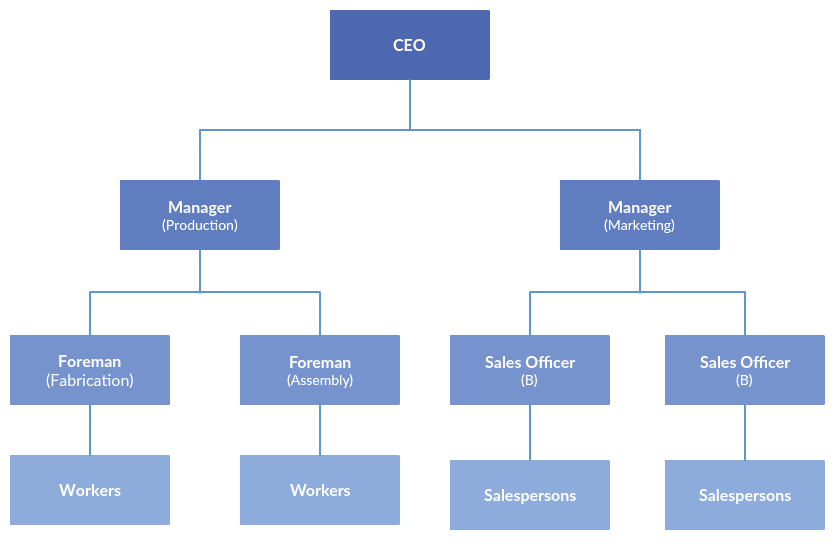
\includegraphics[scale=0.45]{gambar/struktur-organisasi.png}
  % Keterangan gambar yang diinputkan
  \caption{Struktur Organisasi PT. NASA}
  % Label referensi dari gambar yang diinputkan
	\label{fig:strukturOrganisasi}
\end{figure}

% Contoh penggunaan referensi dari gambar yang diinputkan
Seperti yang bisa dilihat pada \ref{fig:strukturOrganisasi}, \lipsum[1]
\vspace{0.5ex}
